% Author: Izaak Neutelings (Februari, 2020)

% page 8 https://archive.org/details/StaticAndDynamicElectricity
% https://tex.stackexchange.com/questions/56353/extract-x-y-coordinate-of-an-arbitrary-point-on-curve-in-tikz
% https://tex.stackexchange.com/questions/412899/tikz-calculate-and-store-the-euclidian-distance-between-two-coordinates

\documentclass[border=3pt,tikz]{standalone}
\usepackage{amsmath} % for \dfrac
\usepackage{bm}
\usepackage{physics}
\usepackage{tikz,pgfplots}
\usepackage[outline]{contour} % glow around text
\pgfplotsset{compat=1.18}
\usetikzlibrary{angles,quotes} % for pic (angle labels)
\usetikzlibrary{decorations.markings}
\usetikzlibrary{shapes,intersections} % for path name
\tikzset{>=latex} % for LaTeX arrow head
\contourlength{1.8pt}

\usepackage{xcolor}
\colorlet{Ecol}{orange!90!black}
\colorlet{EcolFL}{orange!80!black}
\colorlet{veccol}{green!45!black}
\colorlet{EFcol}{red!60!black}
\colorlet{pluscol}{red!60!black}
\colorlet{minuscol}{blue!60!black}
\colorlet{gausscol}{green!50!black!80}
\tikzstyle{charged}=[top color=blue!20,bottom color=blue!40,shading angle=10]
\tikzstyle{charge+}=[very thin,draw=black,top color=red!80,bottom color=red!80!black,shading angle=-5]
\tikzstyle{charge-}=[very thin,draw=black,top color=blue!50,bottom color=blue!70!white!90!black,shading angle=10]
\tikzstyle{darkcharged}=[very thin,top color=blue!60,bottom color=blue!80,shading angle=10]
\tikzstyle{gauss surf}=[green!40!black,top color=green!2,bottom color=green!80!black!70,shading angle=5,fill opacity=0.6]
\tikzstyle{gauss dark}=[green!40!black,fill=green!40!black!70,fill opacity=0.8]
\tikzstyle{gauss line}=[green!40!black]
\tikzstyle{gauss dashed line}=[green!60!black!80,dashed,line width=0.2]
\tikzstyle{vector}=[->,thick,veccol]
\tikzstyle{normalvec}=[->,thick,blue!80!black!80]
\tikzstyle{EField}=[->,thick,Ecol]
\tikzstyle{EField dashed}=[dashed,Ecol,line width=0.6]
\tikzset{
  EFieldLine/.style={thick,EcolFL,decoration={markings,
                     mark=at position #1 with {\arrow{latex}}},
                     postaction={decorate}},
  EFieldLine/.default=0.5}
\tikzstyle{metal}=[top color=black!5,bottom color=black!15,shading angle=30]
\tikzstyle{measure}=[fill=green!70!black!8,midway,outer sep=0,inner sep=1]
\def\L{2.2}
\def\H{2.2}
\def\W{0.30}
\def\Nx{5}
\def\Ny{5}

%\pgfdeclareradialshading{myball}{\pgfpoint{0.5cm}{0cm}}% 
%  {rgb(0cm)=(1,1,1); rgb(0.7cm)=(0.7,0.1,0); rgb(1cm)=(0.5,0.05,0); rgb(1.05cm)=(1,1,1)}


\begin{document}


% NO CHARGE
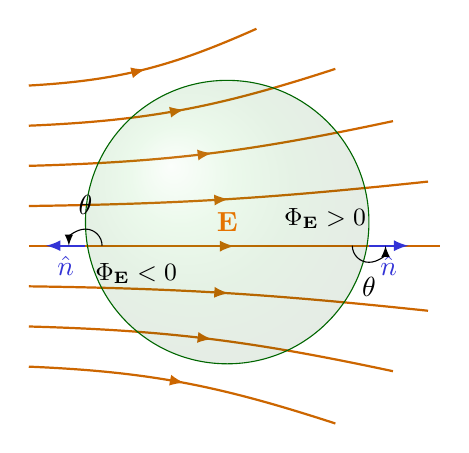
\begin{tikzpicture}
    \def\N{8}
    \def\R{1.8}
    \def\E{6.6}
    \def\r{0.85}

    %% CHARGES
    %\node[charge+,scale=0.8,circle,inner sep=0.24] (C) at (0,0) {$+q$};

    % FIELD LINES
    %\path[name path=ell] (0,0) ellipse ({0.78*\R} and {\R});
    \foreach \i [evaluate={
                \y=0.51*(\i-0.6-\N/2);
                \ang=3.5*(\i-\N/2);
                \out=0.8*(\i-\N/2);
                \in=180+6*(\i-\N/2);
                \r=2.9*\R-0.14*(\i-\N/2)^2;}] in {1,...,\N}{
            \draw[EFieldLine] (-1.4*\R,\y) to[out=\out,in=\in]++ (\ang:\r); %to[out=\out,in=\in]
        }

    % SPHERE
    \draw[gauss line,ball color=green!70!black,fill opacity=0.1]
    (0,0) circle (\R);

    % CHARGE
    \node[below right, font=\small] at (-\R,-0.4) {$\Phi_{\vb{E}} < 0$};
    \node[Ecol] at (0,0) {$\vb{E}$};
    % ANGLE
    \coordinate (A) at (-\R,-0.3);
    \coordinate (B) at (-\R-0.5,-0.3);
    \coordinate (C) at (-\R+0.5,-0.3);

    \draw[normalvec] (A) -- (B) node[midway,below] {$\hat{n}$};
    \draw pic[->,"$\theta$", above, draw=black,angle radius=6,angle eccentricity=1.3] {angle = C--A--B};

    \coordinate (D) at (\R,-0.3);
    \coordinate (E) at (\R+0.5,-0.3);
    \coordinate (F) at (\R-0.5,-0.3);
    \draw[normalvec] (D) -- (E) node[midway,below] {$\hat{n}$};
    \draw pic[->,"$\theta$", below, draw=black,angle radius=6,angle eccentricity=1.3] {angle = F--D--E};
    \node[below right, font=\small] at (\R-1.2,+0.3) {$\Phi_{\vb{E}} > 0$};
\end{tikzpicture}

\end{document}